\section{Interfaces}

\subsection{Mockup}

Figure \ref{fig:mockup} shows a mockup of the team analysis page that was created before starting developing. There are two main sections in the mockup: team statistics and key players.

\begin{figure}[ht!]
\centering
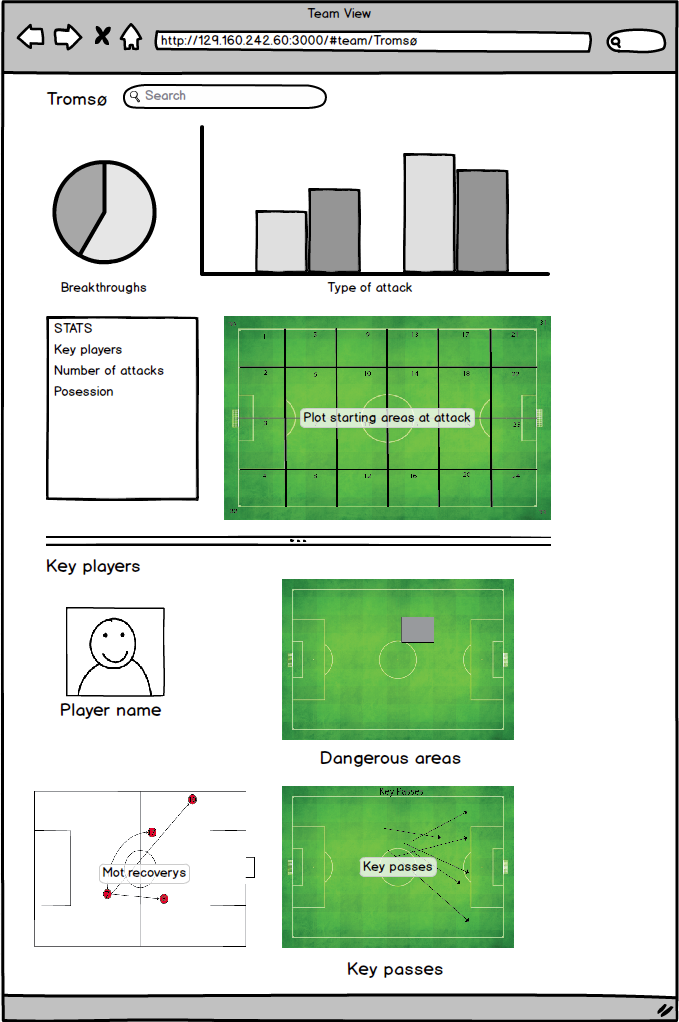
\includegraphics[width=1\textwidth]{images/general/mockup.png}
\caption{A mockup of the main analytic page}
\label{fig:mockup}
\end{figure}

\subsection{Implemented interfaces}

\subsubsection{Home page}
The first page you are prompted with is the listing of all matches registered in the database as figure \ref{fig:all_matches}. A click on match gives you details about that match and prompts you an interface for capturing new attacks if requested. Every field has to be submitted with a correct input value.

\begin{figure}[ht!]
\centering
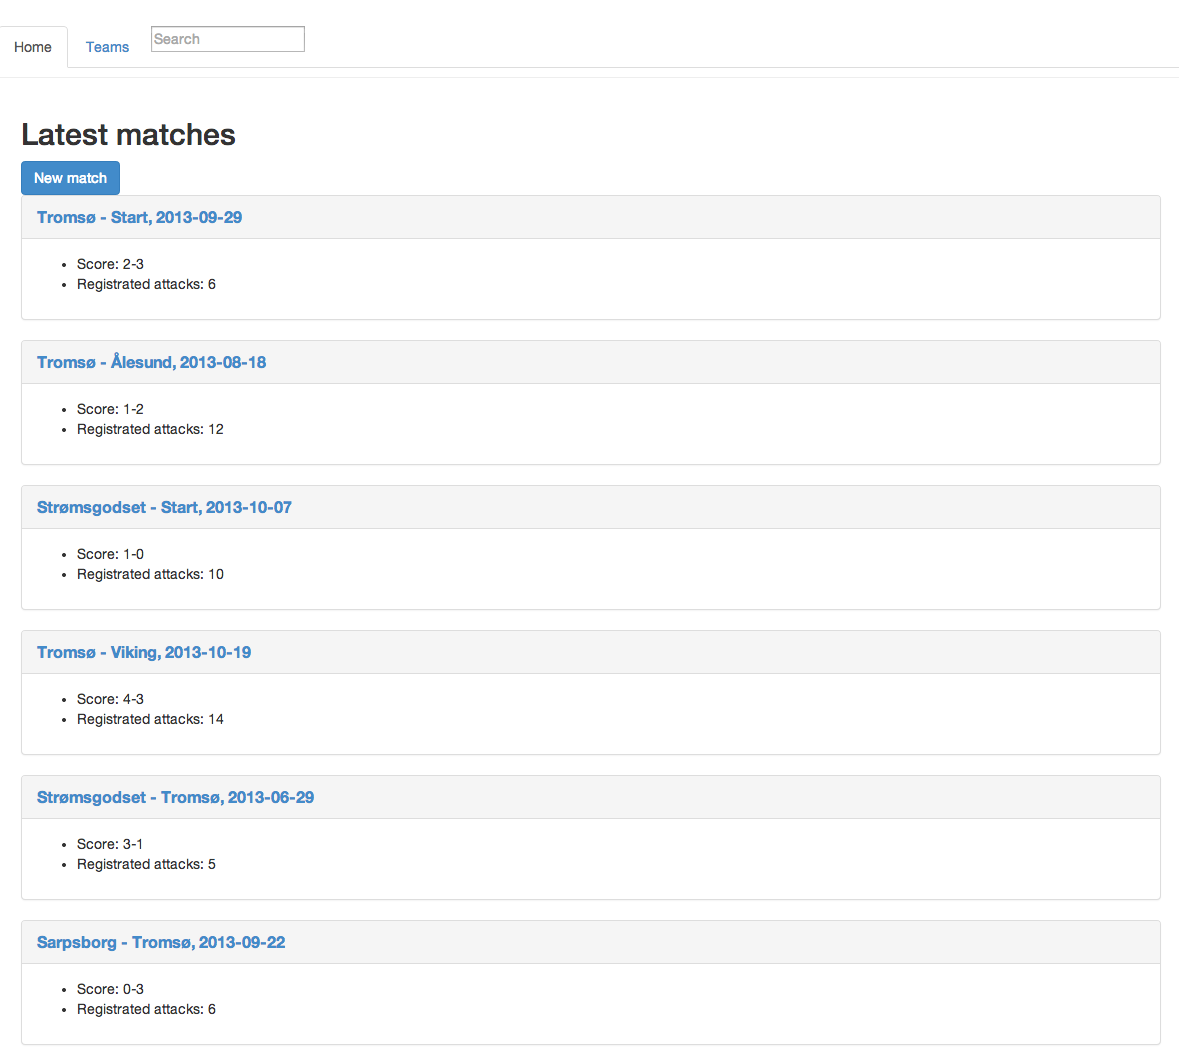
\includegraphics[width=1\textwidth]{images/general/all_matches.png}
\caption{All matches registrated in the database are listed on this page}
\label{fig:all_matches}
\end{figure}

The whole website follows a theme throughout the pages. This theme is the standard theme in the CSS and JavaScript library Bootstrap\footnote{ http://getbootstrap.com/}. Bootstrap makes the website by default responsive. This means the content on the site is automatically re-sized out from the size of your browser window.

\subsubsection{Registrating attacks}
You registrate a new attack by pressing the «New attack» button. Here you fill in the result and date of the match. When you submit the match you will be sent back to the home page. 

\begin{figure}[ht!]
\centering
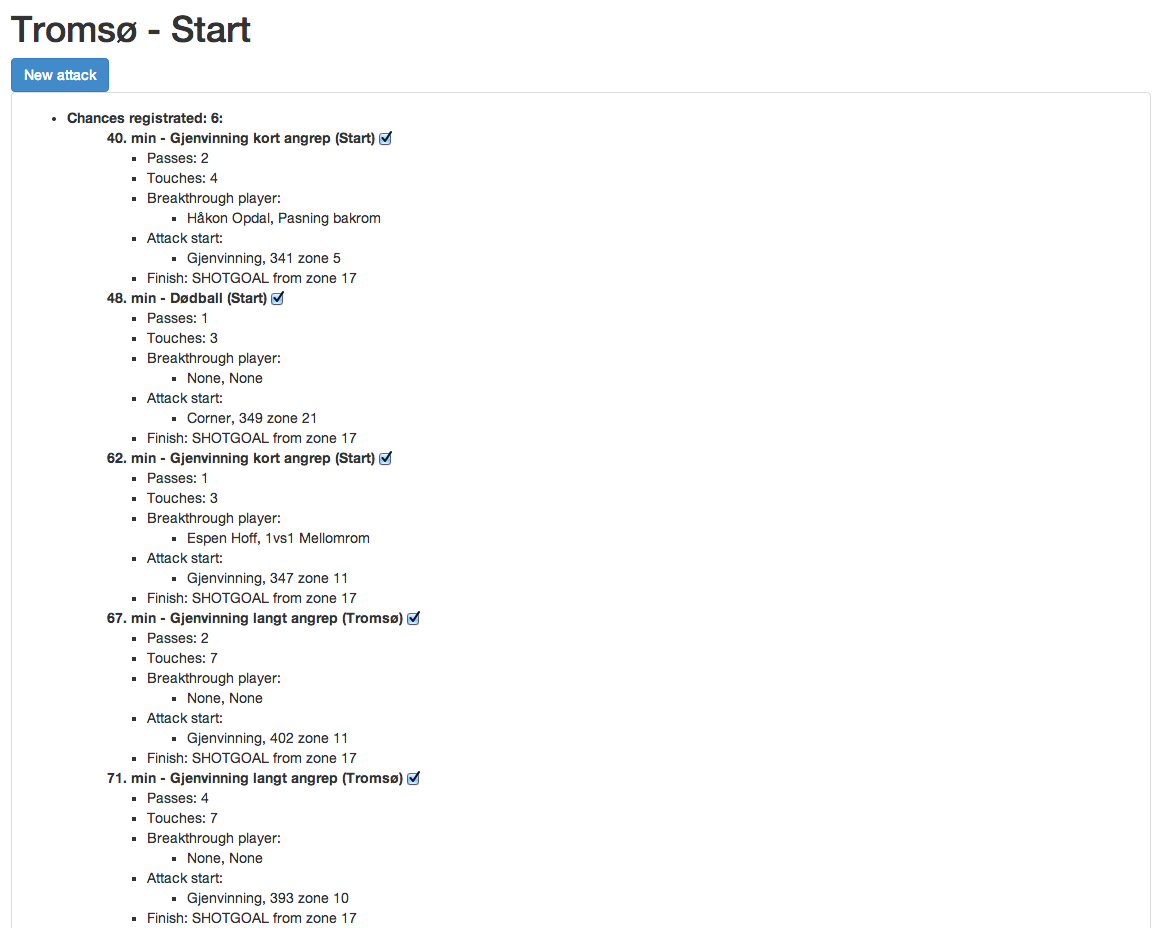
\includegraphics[width=1\textwidth]{images/general/all_attacks.png}
\caption{Interface listing up all attacks for a match}
\label{fig:all_attacks}
\end{figure}

\subsubsection{Match view}

Clicking on a match gives you overview of all attacks registrated for that particular game shown in figure \ref{fig:all_attacks}). This view is only meant for quality checking the data.

From the match page you can add new attack attempts, as figure \ref{fig:reg_attack} shows. This will prompt you with a fill in form for the attack. Attack start, attack end, breakthrough player, time and team needs to be filled out. The passes in the attack are added by pressing new pass. This will add a new pass to the form.

\begin{figure}[ht!]
\centering
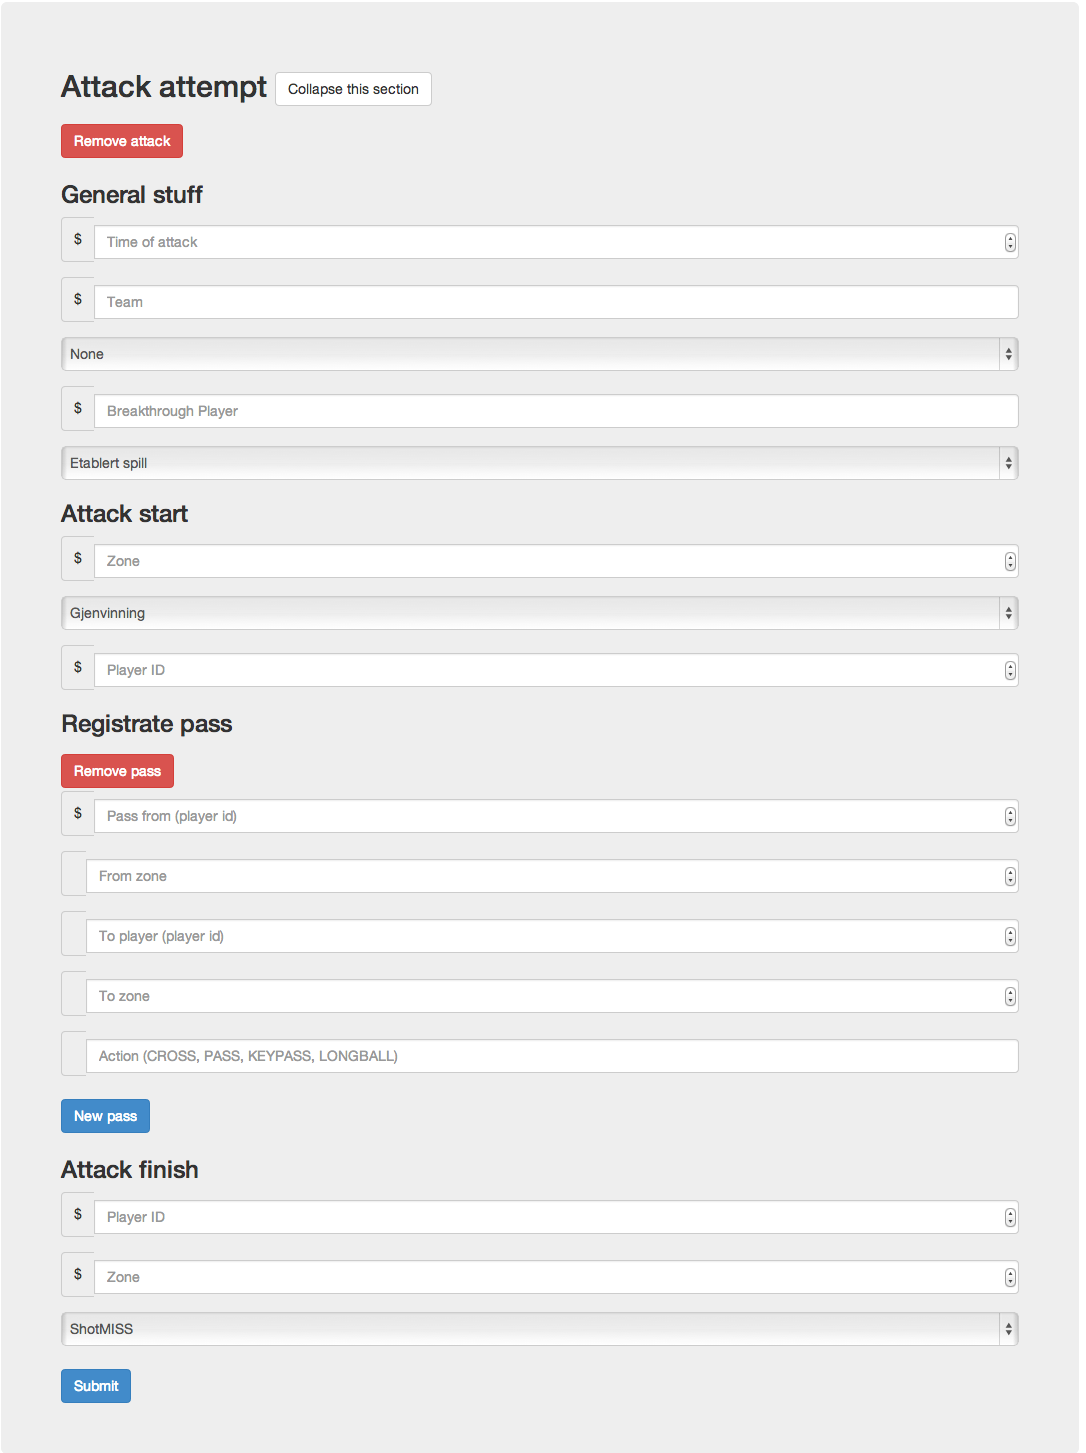
\includegraphics[width=1\textwidth]{images/general/reg_attack.png}
\caption{Interface for registrating an attack}
\label{fig:reg_attack}
\end{figure}

\subsubsection{Team view}

Then you have the team selection page shown in figure \ref{fig:all_teams}). This is a simple layout listing all the teams in the Norwegian premier league. From here you select the team you want to analyze.

\begin{figure}[ht!]
\centering
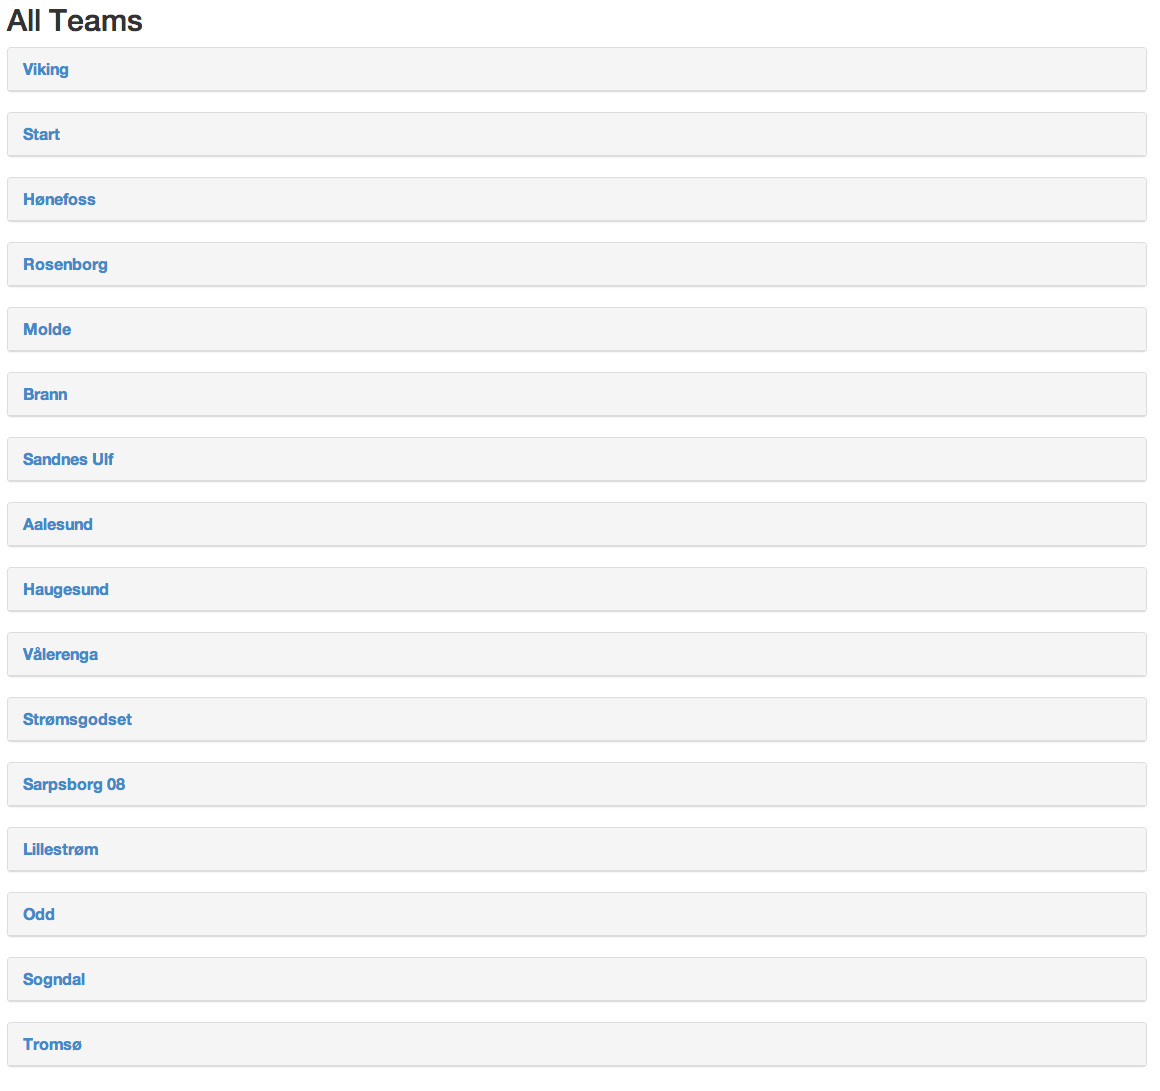
\includegraphics[width=1\textwidth]{images/general/all_teams.png}
\caption{Interface listing all teams}
\label{fig:all_teams}
\end{figure}

Then there is the main view used for analyzing a team, showed in figure \ref{fig:team_analysis1}, figure \ref{fig:team_analysis2} and figure \ref{fig:team_analysis3}. The page design is not exactly the same as the mockup. This comes from a various things. A description of different breakthroughs has been added to enlighten users of the system. Users of the system may or may not have been involved in the process of capturing the data and therefor-extra information is needed to clarify concepts. In the mockup key players where highlighted. In the final view various statistics is presented to the user and he can then click on players he find interesting to know more about as shown in figure \ref{team_analysis4}. The whole page is divided into 3 sections; Key aspects, offensive play, defensive play.

\begin{figure}[ht!]
\centering
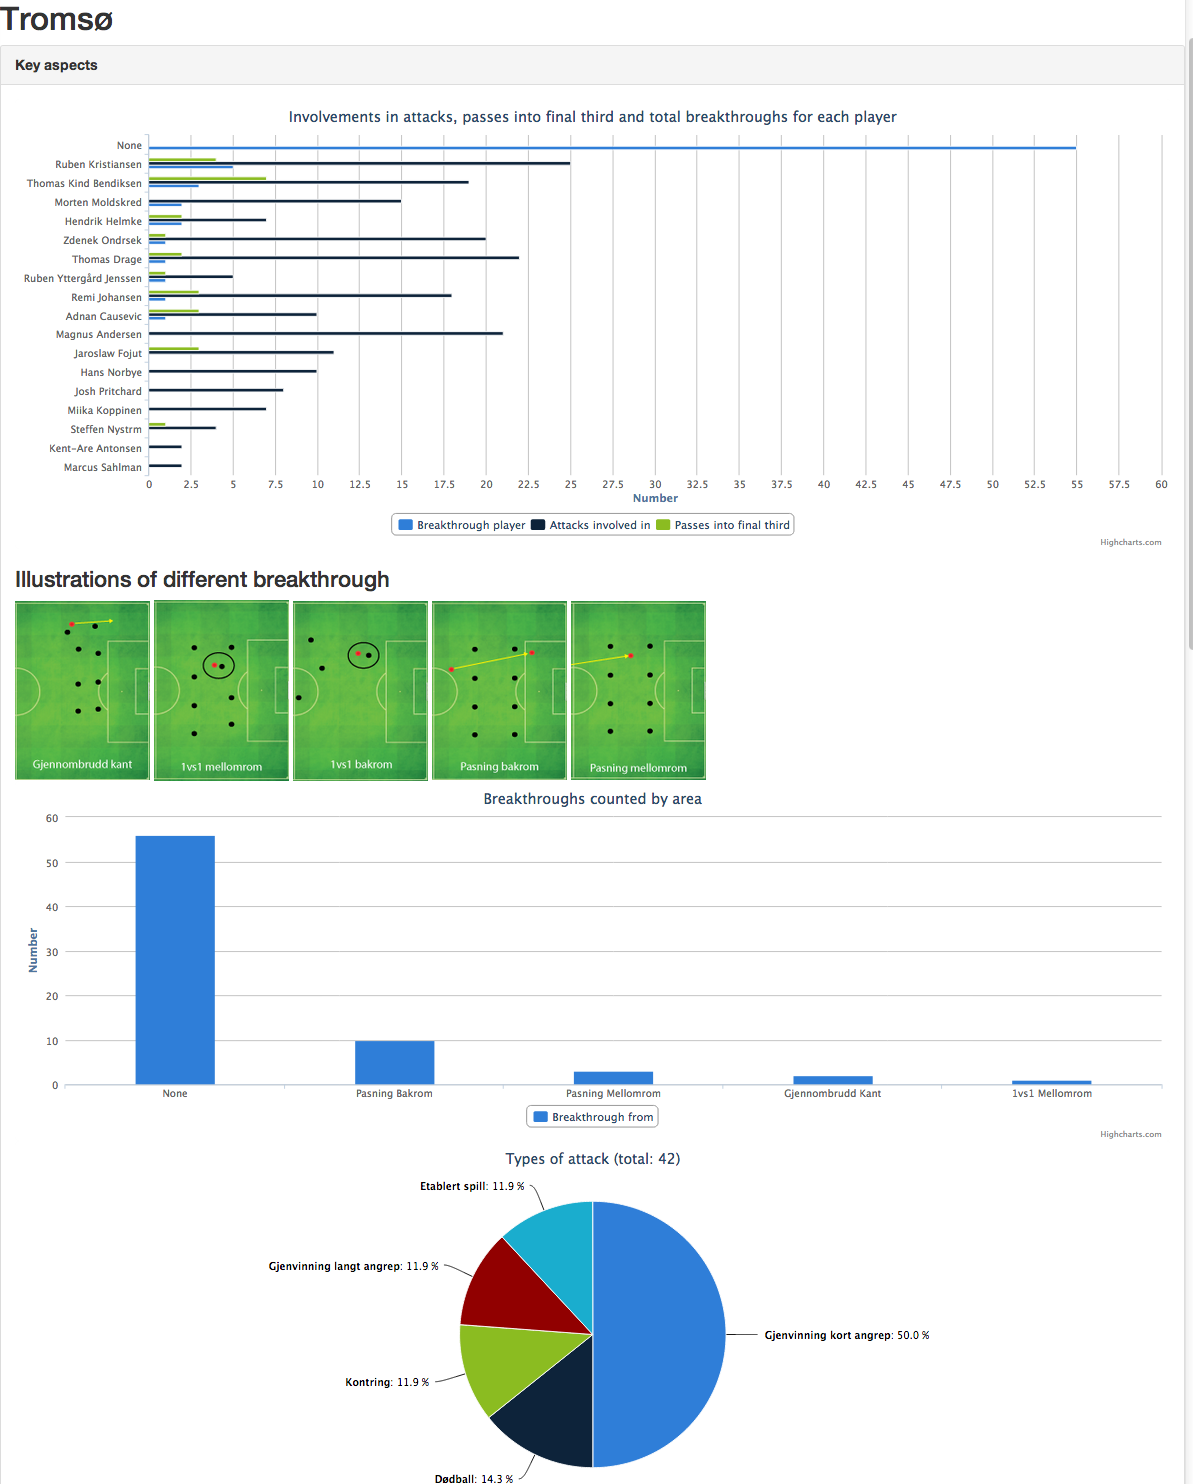
\includegraphics[width=1\textwidth]{images/general/team_analysis1.png}
\caption{Main interface for information about opponents - key aspects}
\label{fig:team_analysis1}
\end{figure}

\begin{figure}[ht!]
\centering
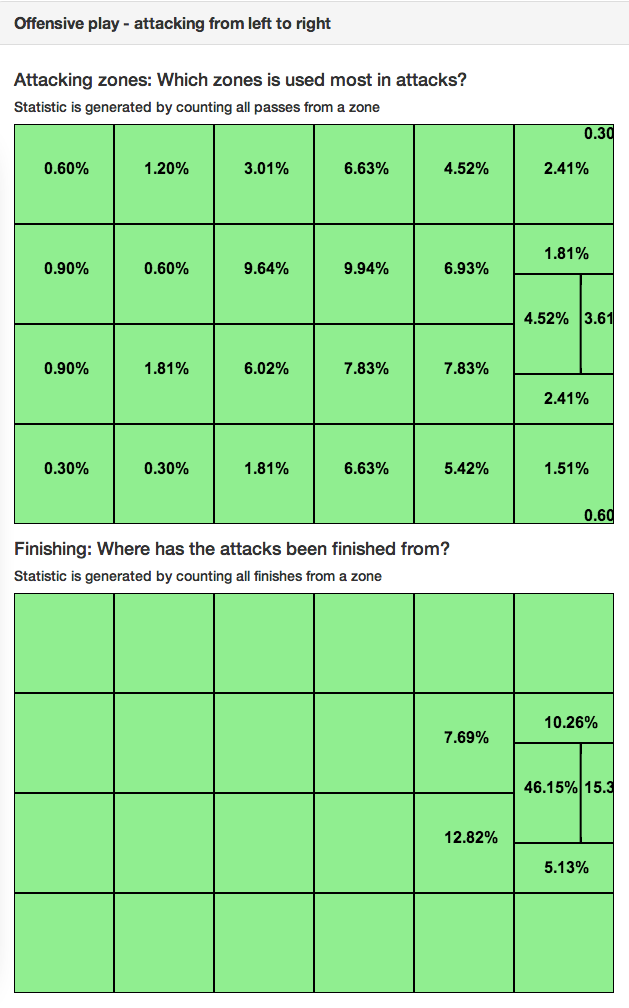
\includegraphics[width=1\textwidth]{images/general/team_analysis2.png}
\caption{Main interface for information about opponents - offensive play}
\label{fig:team_analysis2}
\end{figure}


\begin{figure}[ht!]
\centering
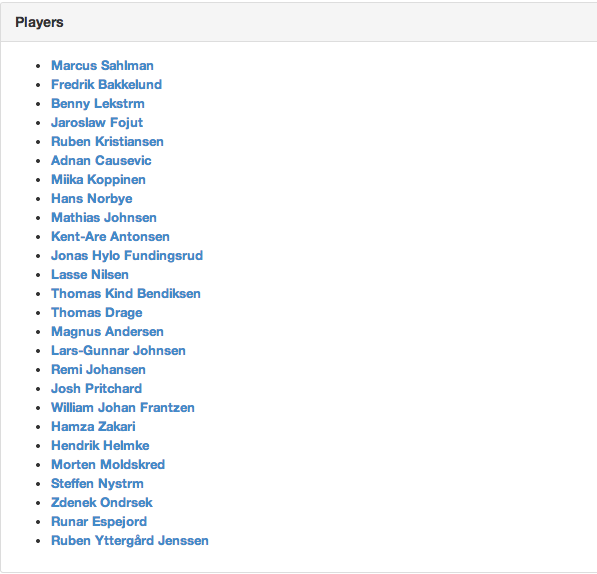
\includegraphics[width=1\textwidth]{images/general/team_analysis3.png}
\caption{Main interface for information about opponents - defensive play‹}
\label{fig:team_analysis3}
\end{figure}

\begin{figure}[ht!]
\centering
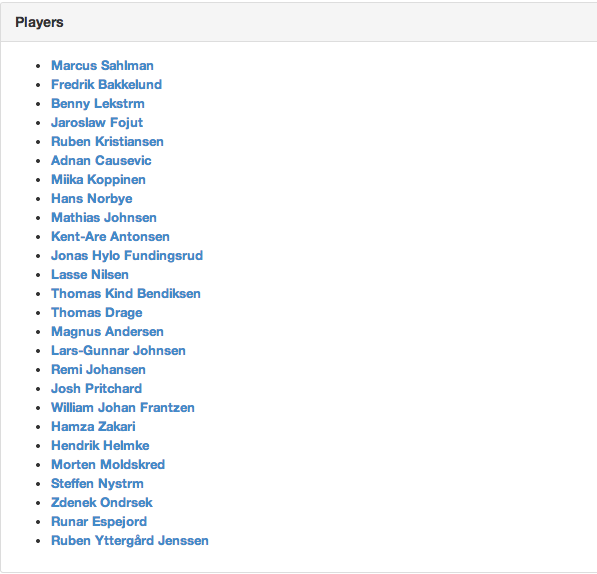
\includegraphics[width=1\textwidth]{images/general/team_analysis4.png}
\caption{Main interface for information about opponents – all players}
\label{fig:team_analysis4}
\end{figure}

Clicking on a player brings you to the player view shown in figure \ref{fig:player_view1} and figure \ref{fig:player_view2}. Here individual statistics is highlighted. 

\begin{figure}[ht!]
\centering
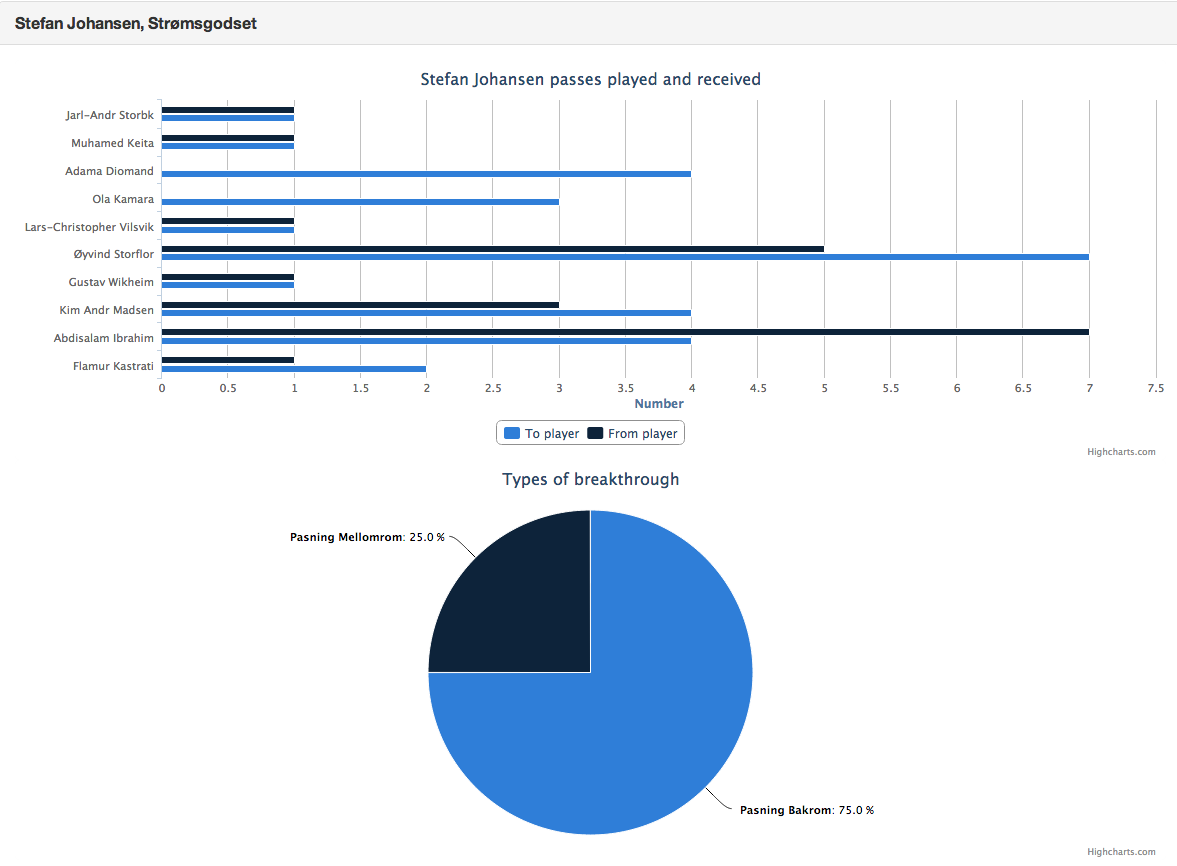
\includegraphics[width=1\textwidth]{images/general/player_view1.png}
\caption{Player view highlighting individual statistics}
\label{fig:player_view1}
\end{figure}

\begin{figure}[ht!]
\centering
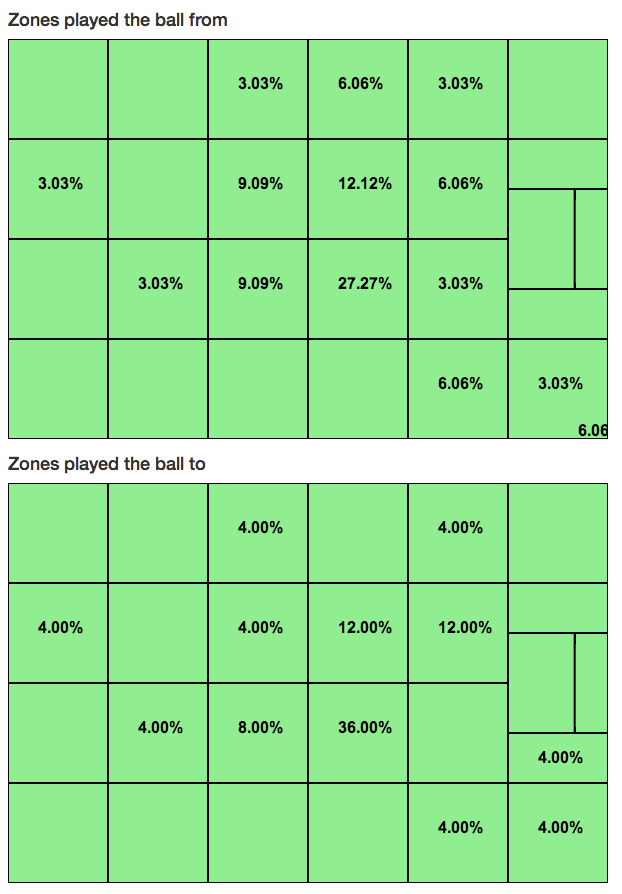
\includegraphics[width=1\textwidth]{images/general/player_view2.png}
\caption{Player view highlighting individual statistics}
\label{fig:player_view2}
\end{figure}


\section{Capturing process}
\label{sec:capprocess}

As mentioned, the process of capturing data is manually. In the beginning it took up to 1 hour to capture all attacks for a match. When you get used to the interface and is able to quickly identify players the time used went down 15-20 minutes. Where most of the time went was getting the players id by looking up in the database manually. 

The process of capturing has been the following:
\begin{enumerate}
\item Download the match video.
\item Find the match in the VGLive.no archives. VGLive.no is used to quickly find all attacks ending with a finish
\item Capture all the attack one by one via the implemented interface mentioned earlier.
\end{enumerate}

